\section{IMU}
The IMU \ref{trm::imu} that was present on WTR before, the MPU6050, was broken when the current group started work on the project.
As such, a replacement had to be chosen.
Rather than go with a 6-axis IMU like the MPU6050, a 9-axis IMU seemed like the better option, so an analysis was done to determine the best device.

The demands were as follows:
\begin{enumerate}
\item Device must have an accelerometer, gyroscope and magnetometer
\item Device must be Arduino/Pi compatible
\item Device must be affordable within the budget given by the product owner
\item Device must be accurate enough to contribute to the solution
\end{enumerate}

The following devices were selected as potentially viable options:
\begin{enumerate}
\item \href{https://www.sparkfun.com/products/13762}{MPU9250}- Sparkfun breakout
\item \href{https://store.arduino.cc/9-axis-motion-shield}{BNO055} - Arduino motionshield
\item \href{https://learn.adafruit.com/nxp-precision-9dof-breakout/overview}{NXP} - Adafruit breakout
\end{enumerate}

Each device has its features outlined in the following table:

\begin{figure}[H]
    \begin{tabular}{|c|c|c|c|c|c|}
    \hline
    \textbf{device} & \textbf{cost} & \textbf{operating voltage $V$} & \textbf{angular scale $^O /sec$} & \textbf{acceleration scale $G$}  & \textbf{format} \\ \hline
    MPU9250 & \$ 14,95 & 2.4 - 3.6 & 250 - 2000 & 2 - 16 & breakout board \\ \hline
    BNO055  & \$ 23,95 & 2.4 - 3.6 & 250 - 2000 & 2 - 16 & Arduino Shield \\ \hline
    NXP     & \$ 14,95 & 2 - 3.6   & 250 - 2000 & 2 - 8   & breakout board \\ \hline
    \end{tabular}
\caption{comparison of features of the three selected 9-axis IMU's}
\label{tbl::IMUcomp}
\end{figure}

The three sensors here are fairly similar, though there are a few critical differences.
The MPU9250 and the NXP are very similar, and even have the same price.
Out of those 2, the MPU has a slightly higher range in the acceleration scale category, which for no added price, meaning it knocks out the NXP.
The MPU9250 and the BNO055 have the same sensitivity, but the price of the BNO055 is significantly higher than the MPU9250.
Therefore, the logical conclusion is that the MPU9250 should be used.

Figures were obtained from the following places:
\begin{itemize}
\item MPU9250 - \cite{mpu}
\item BNO055  - \cite{bno}
\item NXP - \cite{nxp1} , \cite{nxp2}
\end{itemize}


\subsection{Hardware Setup}
The wiring for the MPU9250 is as follows:

\begin{figure}[H]
\centering
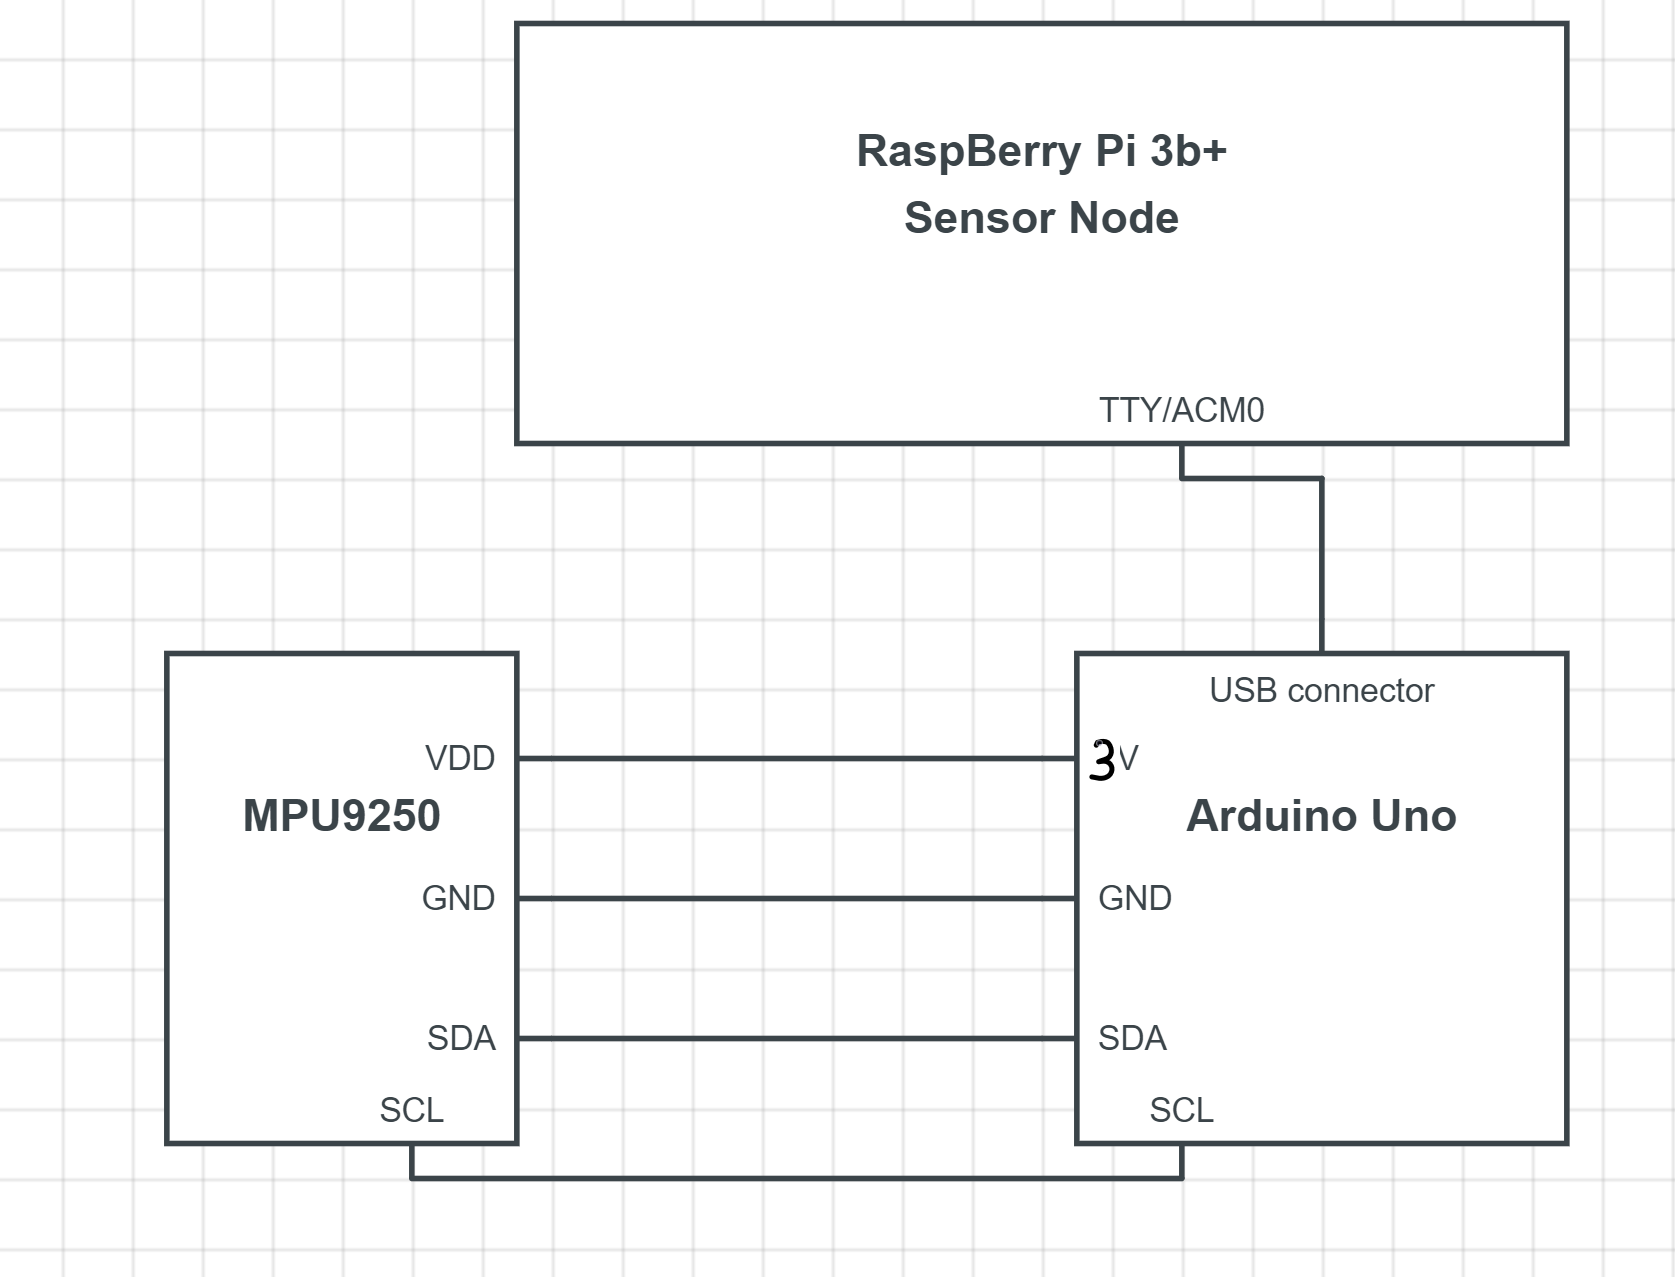
\includegraphics[width=12cm]{wires.png}
\caption{Wiring setup for the MPU to Arduino communication}
\label{fig::wiring}
\end{figure}

The pins used on the arduino are as follows: 
\begin{figure}[H]
\centering
\begin{tabular}{|c|c|}
\hline
\textbf{Pin} & \textbf{Function} \\ \hline
Analogue 4 & SDA \\ \hline
Analogue 5 & SCL \\ \hline
GND        & ground  \\ \hline
3.3V       & VDD     \\ \hline
\end{tabular}
\end{figure}

\subsubsection{Address}
In the example code it is stated the the address of the MPU9250 should be \code{0x71}.
This is not the case, and instead the address is \code{0x73}.
The reason for this difference is not exactly clear, but it does not pose any problem other than the code used not matching the examples.
The magnetometer, the AK8963, does still have the same address as mentioned in any documentation about it, as well as the example code.

\subsubsection{Positioning}
During the development, a small issue was forgotten.
When the word "small" is used, this is an understatement.
A magnetometer is reliant on, as the name implies, magnetism.
Since the frame is made of steel, it interferes with the magnetometer to a rather large extent.
When the IMU is mounted to the frame, the quaternion it outputs is essentially always the same, since the magnetic values never change.
If the robot turns, the magnetic field it produces turns with it.
This is akin to using a compass with a powerful magnet held in front of it.
Regardless of how you turn, the compass will always point towards the magnet, rather than the north.
To combat this issue, there are two solutions.
The first would be to somehow isolate the frame, electric motors and car batteries so that the magnetic field is contained.
No one in the current group has the expertise or knowledge to do this, and it would probably also weigh down WTR so much the robot would become nearly immovable.
The second option is to move the sensor as far away from the source of the interference as possible.
To this end, a case has been designed which can be hung from the top of the screen, as far away from the magnetic influences of the robot as possible.
\newpage    
    